\section*{The 34th International Physics Olympiad}

\begin{center}
\emph{Translated and edited by Zheng Yongling and Jiang Zuimin, Fudan University}
\end{center}

\subsection*{Theoretical Problems}

\begin{problem}{1}
\emph{A pendulum with a falling bob.}

A rigid cylinder of radius $R$ is mounted horizontally above the ground. A bob of mass $m$ is suspended by a string of length $L$ ($L>2\pi R$) and negligible mass from the point $A$ at the top of the cylinder, as shown in Fig.~34.1. The bob is pulled aside until it is on the same horizontal level as $A$, with the string taut, and is then released from rest. Any stretching of the string may be neglected. The bob may be regarded as a particle and moves only in the vertical plane perpendicular to the axis of the cylinder. For this reason the bob is sometimes also called a ``particle''. The acceleration due to gravity is $g$.

As shown in Fig.~34.1, take $O$ as the origin of coordinates. When the particle has descended to the point $P$, the string is tangent to the surface of the cylinder at $Q$. The length of the segment $QP$ is denoted by $s$. At $Q$ the unit vector in the tangential direction is $\hat{t}$, and the unit vector in the radial direction is $\hat{r}$. Take the vertical line along $OA$, pointing upwards, as the $x$ axis; when $OA$ rotates counterclockwise to $OQ$, its angular displacement $\theta$ is taken as positive.

When $\theta=0$, the length of the segment $s$ equals $L$, and the gravitational potential energy $U$ of the particle is set equal to zero. Because of the motion of the particle, the instantaneous rates of change of $\theta$ and $s$ with time are denoted by $\dfrac{d\theta}{dt}$ and $\dfrac{ds}{dt}$, respectively.

Unless otherwise stated, all speeds and velocities are relative to the fixed point $O$.

\textbf{Part A}

In part A only the motion of the particle while the string is taut is considered. Using the quantities given above (namely $s$, $\theta$, $\dfrac{ds}{dt}$, $\dfrac{d\theta}{dt}$, $R$, $L$, $g$, $\hat{t}$, $\hat{r}$), find:

\begin{enumerate}[label=(\alph*),leftmargin=2.2em,itemsep=1pt]
\item the relation between $\dfrac{d\theta}{dt}$ and $\dfrac{ds}{dt}$;
\item the velocity $\vec{v}_Q$ of the moving point $Q$ relative to $O$;
\item when the particle is at $P$, its velocity $\vec{v}'$ relative to the moving point $Q$;
\item when the particle is at $P$, its velocity $\vec{v}$ relative to $O$;
\item when the particle is at $P$, the component in the direction $\hat{t}$ of its acceleration relative to $O$;
\item when the particle is at $P$, its gravitational potential energy $U$;
\item the speed $v_m$ of the particle at the lowest point of its trajectory.
\end{enumerate}

\textbf{Part B}

In part B the ratio of $L$ to $R$ is
\[
\frac{L}{R}=\frac{9\pi}{8}+\frac{2}{3}\cot\frac{\pi}{16}=3.534+3.352=6.886 .
\]

\begin{enumerate}[label=(\alph*),leftmargin=2.2em,itemsep=1pt,start=8]
\item When the string from $Q$ to $P$ is straight and its length is shortest, what is the speed $v_t$ of the particle? (Express it in terms of $g$ and $R$.)
\item When the particle has swung to the other side of the cylinder and reached the highest point, what is its speed $v_H$? (Express it in terms of $g$ and $R$.)
\end{enumerate}

\textbf{Part C}

In part C the bob of mass $m$ is not suspended from $A$; instead, a string passes over the top of the cylinder and is joined on the other side to a heavier object of mass $M$, as shown in Fig.~34.2. This heavy object may also be regarded as a particle.

Initially the bob is pulled to the same horizontal level as $A$, while the heavy object at the other end hangs below the point $O$; the string is taut and the length of its horizontal part is $L$. The bob is then released from rest, and the heavy object begins to fall. Assume that the bob remains in the vertical plane and can swing past the vertically hanging heavy object and string without colliding with them.

The kinetic friction between the string and the surface of the cylinder is negligible, but the static friction is large enough that, once the speed of the falling heavy object has become zero, the object can be held at rest.

\begin{enumerate}[label=(\alph*),leftmargin=2.2em,itemsep=1pt,start=10]
\item Suppose that after the heavy object has fallen a distance $D$ its speed becomes zero, and that $L-D\gg R$. If the bob can thereafter swing around the cylinder to $\theta=2\pi$ while the two free segments of the string remain straight, then the ratio $\alpha=D/L$ must be not less than a certain value $\alpha_c$. Neglecting terms of order $R/L$ and higher, estimate the critical value $\alpha_c$ (express it in terms of $M/m$).
\end{enumerate}

\begin{figbox}{34.1}
\begin{tikzpicture}[x=1.35cm,y=1.35cm,line join=round]
  \def\R{1.15}
  \coordinate (O) at (0,0);
  \coordinate (Q) at (-0.881,0.739);
  \coordinate (P) at (-2.616,-1.329);
  \draw[thickline] (O) circle (\R);
  \draw[axis] (0,-\R-0.10) -- (0,\R+0.55);
  \node[left,font=\small] at (0,\R+0.50) {$x$};
  % initial position of the string
  \draw[thickline] (-3.704,1.15) -- (0,1.15);
  \fill (-3.704,1.15) circle (1.6pt);
  \node[left,font=\small] at (-3.704,1.15) {$m$};
  \node[above,font=\small] at (-1.85,1.17) {$L$};
  % string at the later instant
  \draw[thickline] (Q) -- (P);
  \draw[fill=white] (P) circle (1.5pt);
  \node[below left,font=\small] at (P) {$P$};
  \draw[fill=white] (Q) circle (1.5pt);
  \node[above right,font=\small] at (Q) {$Q$};
  \node[right,font=\small] at (0,1.15) {$A$};
  % radius
  \draw[thickline] (O) -- (1.15,0);
  \node[above,font=\small] at (0.80,0.03) {$R$};
  \node[below left,font=\small] at (0,0) {$O$};
  % angle theta
  \draw (0,0.55) arc[start angle=90,end angle=140,radius=0.55];
  \node[font=\small] at (-0.50,0.62) {$\theta$};
  % unit vectors
  \draw[force] (Q) -- ++(-0.45,-0.536);
  \node[below right,font=\small] at (-1.30,-0.10) {$\hat{t}$};
  \draw[force] (Q) -- ++(-0.46,0.386);
  \node[left,font=\small] at (-1.58,1.10) {$\hat{r}$};
  \node[above right,font=\small] at (-1.98,-0.38) {$s$};
  % gravity
  \draw[force] (-2.95,0.30) -- (-2.95,-0.28);
  \node[right,font=\small] at (-2.93,-0.02) {$g$};
\end{tikzpicture}
\end{figbox}

\begin{figbox}{34.2}
\begin{tikzpicture}[x=1.30cm,y=1.30cm,line join=round]
  \def\R{1.15}
  \coordinate (O) at (0,0);
  \draw[thickline] (O) circle (\R);
  \draw[thickline] (-3.50,1.15) -- (0,1.15);
  \draw[thickline] (0,1.15) arc[start angle=90,end angle=15,radius=\R];
  \draw[thickline] (1.111,0.298) -- (1.111,-1.42);
  \draw[thickline] (1.02,-1.42) rectangle (1.20,-1.66);
  \node[right,font=\small] at (1.23,-1.54) {$M$};
  \fill (-3.50,1.15) circle (1.6pt);
  \node[left,font=\small] at (-3.50,1.15) {$m$};
  \node[above,font=\small] at (-1.75,1.17) {$L$};
  \draw[thickline] (O) -- (1.15,0);
  \node[below,font=\small] at (0.62,-0.02) {$R$};
  \node[below left,font=\small] at (0,0) {$O$};
  \node[above,font=\small] at (0,1.15) {$A$};
  \draw (15:0.45) arc[start angle=15,end angle=90,radius=0.45];
  \node[font=\small] at (0.38,0.52) {$\theta$};
\end{tikzpicture}
\end{figbox}

\end{problem}

\subsection*{Solutions}

\begin{solution}{1}

\textbf{Part A}

(a) Since the length of the string, $L=s+R\theta$, is constant,\footnote{Equation numbers marked with an asterisk ($^{*}$) denote answers to the problem; the same convention applies below.} we have
\begin{equation}
\frac{ds}{dt}+R\frac{d\theta}{dt}=0 . \tag{A1$^{*}$}
\end{equation}

(b) Relative to $O$, the point $Q$ moves on a circle of radius $R$ with angular velocity $\dfrac{d\theta}{dt}$; hence
\begin{equation}
\vec{v}_Q=R\frac{d\theta}{dt}\,\hat{t}=-\frac{ds}{dt}\,\hat{t}. \tag{A2$^{*}$}
\end{equation}

(c) Relative to $Q$, the displacement of the particle during the time interval $\Delta t$ is
\[
\Delta\vec{r}'=(s\,\Delta\theta)(-\hat{r})+\Delta s\,\hat{t}.
\]
See Fig.~34.3. Hence
\begin{equation}
\vec{v}'=\frac{\Delta\vec{r}'}{\Delta t}=-s\frac{d\theta}{dt}\,\hat{r}+\frac{ds}{dt}\,\hat{t}. \tag{A3$^{*}$}
\end{equation}

(d) The velocity of the particle relative to $O$ is the sum of the two velocities given by (A2) and (A3); therefore
\begin{equation}
\vec{v}=\vec{v}'+\vec{v}_Q=-s\frac{d\theta}{dt}\,\hat{r}+\frac{ds}{dt}\,\hat{t}-\frac{ds}{dt}\,\hat{t}
=-s\frac{d\theta}{dt}\,\hat{r}. \tag{A4$^{*}$}
\end{equation}

\begin{figbox}{34.3}
\begin{tikzpicture}[x=1.45cm,y=1.30cm,line join=round]
  \coordinate (Q) at (0,0);
  \coordinate (P) at (-1.838,-1.838);
  \coordinate (Pp) at (-1.417,-2.181);
  \coordinate (Ppp) at (-1.608,-2.475);
  \draw[thickline] (Q) -- (P);
  \draw[dashedline] (Q) -- (Ppp);
  \draw[thickline] (P) -- (Pp);
  \draw[thickline] (Pp) -- (Ppp);
  \draw[force] (P) -- (Ppp);
  \fill (Q) circle (1.4pt) node[above right,font=\small] {$Q$};
  \fill (P) circle (1.2pt);
  \node[below left,font=\small] at (P) {$P$};
  \fill (Ppp) circle (1.2pt);
  \node[below,font=\small] at (Ppp) {$P'$};
  \node[above left,font=\small] at (-0.95,-0.80) {$s$};
  \node[right,font=\small] at (-0.80,-1.55) {$s+\Delta s$};
  \node[below,font=\small] at (-1.60,-2.05) {$s\Delta\theta$};
  \node[below right,font=\small] at (-1.52,-2.50) {$\Delta s$};
  \node[right,font=\small] at (-1.34,-2.14) {$\Delta\vec{r}'$};
  \draw (225:0.55) arc[start angle=225,end angle=237,radius=0.55];
  \node[font=\small] at (-0.52,-0.62) {$\Delta\theta$};
  \draw[force] (P) -- ++(-0.354,-0.354);
  \node[below left,font=\small] at (-2.27,-2.25) {$\hat{t}$};
  \draw[force] (P) -- ++(-0.354,0.354);
  \node[left,font=\small] at (-2.28,-1.52) {$\hat{r}$};
\end{tikzpicture}
\end{figbox}

\begin{figbox}{34.4}
\begin{tikzpicture}[x=1.55cm,y=1.25cm,line join=round]
  \coordinate (O) at (0,0);
  \coordinate (Q) at (-0.35,2.20);
  \coordinate (P) at (0.45,2.05);
  \coordinate (T) at (-0.20,0.40);
  \coordinate (A) at (0.005,-0.883);
  \coordinate (B) at (-0.461,-0.786);
  \draw[dashedline] (O) -- ($(Q)+(0.010,-0.06)$);
  \draw[dashedline] (O) -- ($(P)+(0.020,-0.09)$);
  \draw (O) ++(77.6:0.75) arc[start angle=77.6,end angle=99.0,radius=0.75];
  \node[font=\small] at (0.10,0.78) {$\Delta\theta$};
  \fill (Q) circle (1.4pt) node[above,font=\small] {$Q$};
  \fill (P) circle (1.4pt) node[right,font=\small] {$P$};
  \draw[force] (Q) -- ++(0.44,0.07);
  \node[right,font=\small] at (0.16,2.37) {$\hat{t}$};
  \draw[force] (Q) -- ++(-0.09,0.56);
  \node[left,font=\small] at (-0.50,2.82) {$\hat{r}$};
  % velocity triangle
  \draw[force] (T) -- (A);
  \node[right,font=\small] at (0.10,-0.30) {$\vec{v}$};
  \draw[force] (T) -- (B);
  \node[left,font=\small] at (-0.66,-0.30) {$\vec{v}+\Delta\vec{v}$};
  \draw[force] (A) -- (B);
  \node[below,font=\small] at (-0.28,-0.98) {$\Delta\vec{v}$};
  \draw (T) ++(-80.8:0.30) arc[start angle=-80.8,end angle=-98.8,radius=0.30];
\end{tikzpicture}
\end{figbox}

(e) Referring to Fig.~34.4, the component of the velocity change $\Delta\vec{v}$ in the $(-\hat{t})$ direction is given by
\[
(-\hat{t})\cdot\Delta\vec{v}=v\,\Delta\theta=v\frac{d\theta}{dt}\,\Delta t .
\]
Hence the $\hat{t}$ component of the acceleration $\vec{a}=\Delta\vec{v}/\Delta t$ is
$\hat{t}\cdot\vec{a}=-v\dfrac{d\theta}{dt}$. From (A4) the speed of the particle is $s\dfrac{d\theta}{dt}$; therefore the $\hat{t}$ component of the acceleration of the particle at $P$ is
\begin{equation}
a_t=\vec{a}\cdot\hat{t}=-v\frac{d\theta}{dt}=-\left(s\frac{d\theta}{dt}\right)\frac{d\theta}{dt}
=-s\left(\frac{d\theta}{dt}\right)^2 . \tag{A5$^{*}$}
\end{equation}

Note that, from Fig.~34.4, the radial component of the acceleration of the particle can also be obtained in a similar way:
\[
a_r=\vec{a}\cdot\hat{r}=-\frac{dv}{dt}=-\frac{d}{dt}\left(s\frac{d\theta}{dt}\right).
\]

\begin{figbox}{34.5}
\begin{tikzpicture}[x=1.42cm,y=1.42cm,line join=round]
  \def\R{1.15}
  \coordinate (O) at (0,0);
  \draw[thickline] (O) circle (\R);
  \draw[dashedline] (-2.45,1.15) -- (0.18,1.15);
  \draw[dashedline] (-2.45,-1.30) -- (0.18,-1.30);
  \draw[dashedline] (-2.45,1.15) -- (-2.45,-1.30);
  \draw[dashedline] (0.18,1.15) -- (0.18,-1.30);
  \draw[axis] (0,-1.36) -- (0,1.55);
  \node[left,font=\small] at (0,1.50) {$x$};
  \draw[thickline] (-0.942,0.660) -- (-2.204,-1.142);
  \fill (0,1.15) circle (1.3pt) node[right,font=\small] {$A$};
  \fill (-0.942,0.660) circle (1.3pt) node[above right,font=\small] {$Q$};
  \fill (-2.204,-1.142) circle (1.3pt) node[below,font=\small] {$P$};
  \fill (O) circle (1.1pt) node[below right,font=\small] {$O$};
  \draw[dim] (-2.62,1.15) -- (-2.62,-1.142);
  \node[left,font=\small] at (-2.64,0.00) {$h$};
  \draw[dim] (-2.38,0.660) -- (-2.38,-1.142);
  \node[rotate=90,fill=white,inner sep=1pt,font=\small] at (-2.38,-0.28) {$s\sin\theta$};
  \draw[dim] (1.30,0.660) -- (1.30,1.15);
  \node[right,font=\small] at (1.32,0.90) {$R-R\cos\theta$};
  \draw[dim] (1.30,0) -- (1.30,0.660);
  \node[right,font=\small] at (1.32,0.33) {$R\cos\theta$};
  \draw[thickline] (O) -- (0.941,-0.663);
  \node[below right,font=\small] at (0.50,-0.36) {$R$};
\end{tikzpicture}
\end{figbox}

(f) From Fig.~34.5, the gravitational potential energy of the particle can be expressed in terms of $s$ and $\theta$ as
\begin{equation}
U(\theta)=-mgh=-mg\left[R(1-\cos\theta)+s\sin\theta\right]. \tag{A6$^{*}$}
\end{equation}

\begin{figbox}{34.6}
\begin{tikzpicture}[x=1.45cm,y=1.45cm,line join=round]
  \def\R{1.15}
  \coordinate (O) at (0,0);
  \draw[thickline] (O) circle (\R);
  \draw[axis] (0,-1.45) -- (0,1.45);
  \node[left,font=\small] at (0,1.40) {$x$};
  \fill (0,1.15) circle (1.3pt) node[right,font=\small] {$A$};
  \draw[thickline] (O) -- (-1.15,0);
  \node[below,font=\small] at (-0.58,-0.04) {$R$};
  \fill (-1.15,0) circle (1.3pt) node[above right,font=\small] {$Q$};
  \draw[thickline] (-1.15,0) -- (-1.15,-1.32);
  \node[left,font=\small] at (-1.17,-0.70) {$s$};
  \fill (-1.15,-1.32) circle (1.3pt);
  \node[below,font=\small,align=center] at (-1.15,-1.36) {$P$ (at rest)};
  \fill (O) circle (1.1pt) node[below right,font=\small] {$O$};
\end{tikzpicture}
\end{figbox}

(g) At the lowest point of its trajectory the gravitational potential energy $U$ of the particle must take its minimum value $U_m$. This position of minimum potential energy can be found from the equilibrium position of the particle. It is not difficult to see that it is the position $\theta=\dfrac{\pi}{2}$, i.e. $s=L-\dfrac{\pi R}{2}$ (Fig.~34.6). Hence
\begin{equation}
U_m=U\left(\frac{\pi}{2}\right)=-mg\left(R+L-\frac{\pi R}{2}\right). \tag{A7}
\end{equation}

Initially the mechanical energy of the particle is zero; by conservation of mechanical energy, the speed $v_m$ of the particle at the lowest point of its trajectory must satisfy
\begin{equation}
E=0=\frac{1}{2}mv_m^2+U_m . \tag{A8}
\end{equation}
From (A7) and (A8) we obtain
\begin{equation}
v_m=\sqrt{-\frac{2U_m}{m}}=\sqrt{2g\left[R+\left(L-\frac{\pi R}{2}\right)\right]}. \tag{A9$^{*}$}
\end{equation}

\textbf{Part B}

(h) From (A6), the total mechanical energy of the particle can be written as
\begin{equation}
E=0=\frac{1}{2}mv^2+U(\theta)=\frac{1}{2}mv^2-mg\left[R(1-\cos\theta)+s\sin\theta\right]. \tag{B1}
\end{equation}

From (A4) the speed of the particle is $s\dfrac{d\theta}{dt}$; hence from (B1) we obtain
\begin{equation}
v^2=\left(s\frac{d\theta}{dt}\right)^2=2g\left[R(1-\cos\theta)+s\sin\theta\right]. \tag{B2}
\end{equation}

Let $T$ be the tension in the string. As shown in Fig.~34.7, the $\hat{t}$ component of the net force acting on the particle is $-T+mg\sin\theta$; therefore, by Newton's second law,
\begin{equation}
m\left[-s\left(\frac{d\theta}{dt}\right)^2\right]=-T+mg\sin\theta . \tag{B3}
\end{equation}

From (B2) and (B3) the tension can be expressed as
\begin{align}
T&=m\left[g\sin\theta+s\left(\frac{d\theta}{dt}\right)^2\right]
=\frac{mg}{s}\left[2R(1-\cos\theta)+3s\sin\theta\right]\notag\\
&=\frac{2mgR}{s}\left[\tan\frac{\theta}{2}-\frac{3}{2}\left(\theta-\frac{L}{R}\right)\right]\sin\theta
=\frac{2mgR}{s}(y_1-y_2)\sin\theta \tag{B4}
\end{align}
The curves of the functions $y_1=\tan\dfrac{\theta}{2}$ and $y_2=\dfrac{3}{2}\left(\theta-\dfrac{L}{R}\right)$ are drawn in Fig.~34.8.

\begin{figbox}{34.7}
\begin{tikzpicture}[x=1.45cm,y=1.40cm,line join=round]
  \def\R{1.15}
  \coordinate (O) at (0,0);
  \coordinate (Q) at (-0.881,0.739);
  \coordinate (P) at (-2.616,-1.329);
  \draw[thickline] (O) circle (\R);
  \draw[dashedline] (0,-\R-0.10) -- (0,\R+0.45);
  \draw[axis] (0,\R+0.10) -- (0,\R+0.55);
  \node[left,font=\small] at (0,\R+0.50) {$x$};
  \draw[thickline] (Q) -- (P);
  \fill (Q) circle (1.3pt) node[above right,font=\small] {$Q$};
  \fill (P) circle (1.3pt);
  \node[right,font=\small] at (-2.45,-1.42) {$P$};
  \node[right,font=\small] at (0,1.15) {$A$};
  \draw[thickline] (O) -- (1.15,0);
  \node[above,font=\small] at (0.80,0.03) {$R$};
  \node[below left,font=\small] at (0,0) {$O$};
  \draw (0,0.55) arc[start angle=90,end angle=140,radius=0.55];
  \node[font=\small] at (-0.50,0.62) {$\theta$};
  % tension along the string
  \draw[force] ($(P)!0.55!(Q)$) -- ($(P)!0.85!(Q)$);
  \node[right,font=\small] at (-2.10,-1.02) {$T$};
  % weight and its component
  \draw[force] (P) -- ++(0,-0.55);
  \node[right,font=\small] at (-2.40,-1.80) {$mg$};
  \draw[force] (P) -- ++(-0.45,-0.536);
  \node[below,font=\small] at (-3.02,-1.88) {$mg\sin\theta$};
\end{tikzpicture}
\end{figbox}

\begin{figbox}{34.8}
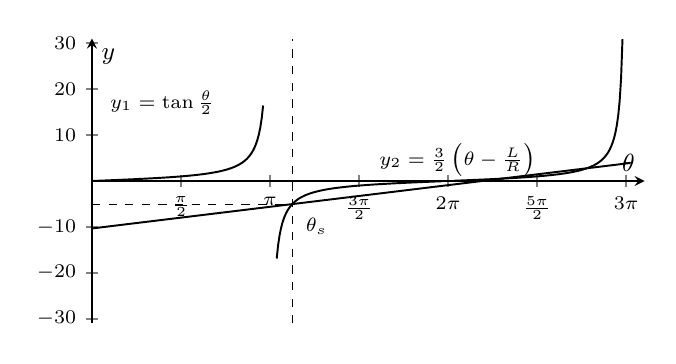
\begin{tikzpicture}
\begin{axis}[
  width=8.6cm,height=5.2cm,
  axis lines=middle,
  xmin=0,xmax=9.75,ymin=-31,ymax=31,
  xtick={0,1.5708,3.1416,4.7124,6.2832,7.8540,9.4248},
  xticklabels={$0$,$\frac{\pi}{2}$,$\pi$,$\frac{3\pi}{2}$,$2\pi$,$\frac{5\pi}{2}$,$3\pi$},
  ytick={-30,-20,-10,0,10,20,30},
  tick label style={font=\scriptsize},
  xlabel={$\theta$},ylabel={$y$},
  xlabel style={font=\small},ylabel style={font=\small},
  axis line style={line width=0.6pt},
  tick style={line width=0.5pt},
  clip=true,
]
\addplot[domain=0:3.02,samples=120,line width=0.7pt] {tan(deg(x/2))};
\addplot[domain=3.26:6.18,samples=120,line width=0.7pt] {tan(deg(x/2))};
\addplot[domain=6.38:9.36,samples=120,line width=0.7pt] {tan(deg(x/2))};
\addplot[domain=0:9.5,samples=2,line width=0.7pt] {1.5*(x-6.886)};
\addplot[dashed,line width=0.4pt] coordinates {(3.534,-31) (3.534,31)};
\addplot[dashed,line width=0.4pt] coordinates {(0,-5.03) (3.534,-5.03)};
\node[font=\scriptsize,anchor=west] at (axis cs:0.15,17) {$y_1=\tan\frac{\theta}{2}$};
\node[font=\scriptsize,anchor=west] at (axis cs:4.9,4.5) {$y_2=\frac{3}{2}\left(\theta-\frac{L}{R}\right)$};
\node[font=\scriptsize,anchor=north west] at (axis cs:3.60,-6.0) {$\theta_s$};
\end{axis}
\end{tikzpicture}
\end{figbox}

\begin{center}
\small Table 34.1
\end{center}
\begin{center}
\begin{tabular}{cccc}
\toprule
 & $y_1-y_2$ & $\sin\theta$ & Tension $T$\\
\midrule
$0<\theta<\pi$ & positive & positive & positive\\
$\theta=\pi$ & $+\infty$ & $0$ & positive\\
$\pi<\theta<\theta_s$ & negative & negative & positive\\
$\theta=\theta_s$ & zero & negative & zero\\
$\theta_s<\theta<2\pi$ & positive & negative & negative\\
\bottomrule
\end{tabular}
\end{center}

From (B4) and Fig.~34.8 the results listed in Table 34.1 are obtained. Let $\theta_s$ ($\pi<\theta_s<2\pi$) denote the angle at which $y_2=y_1$; it is given by
\begin{equation}
\frac{3}{2}\left(\theta_s-\frac{L}{R}\right)=\tan\frac{\theta_s}{2}, \tag{B5}
\end{equation}
or
\begin{equation}
\frac{L}{R}=\theta_s-\frac{2}{3}\tan\frac{\theta_s}{2}. \tag{B6}
\end{equation}
Since the ratio $L/R$ is given by
\begin{equation}
\frac{L}{R}=\frac{9\pi}{8}+\frac{2}{3}\cot\frac{\pi}{16}
=\left(\pi+\frac{\pi}{8}\right)-\frac{2}{3}\tan\frac{1}{2}\left(\pi+\frac{\pi}{8}\right), \tag{B7}
\end{equation}
equations (B6) and (B7) give
\[
\theta_s=\frac{9\pi}{8}.
\]

From Table 34.1 it is seen that the tension $T$ is always positive in the range $0<\theta<\theta_s$ (that is, the string must remain taut). As soon as $\theta$ reaches $\theta_s$ the tension becomes zero, and thereafter the free part of the string will no longer be taut. The smallest possible value $s_{\min}$ of $s$ occurs at $\theta=\theta_s$ and is given by
\begin{equation}
s_{\min}=L-R\theta_s=R\left(\frac{9\pi}{8}+\frac{2}{3}\cot\frac{\pi}{16}-\frac{9\pi}{8}\right)
=\frac{2R}{3}\cot\frac{\pi}{16}=3.352R . \tag{B8}
\end{equation}

When $\theta=\theta_s$, $T=0$; from (B2) and (B3) we obtain $v^2=-gs\sin\theta$, so the speed $v_t$ is
\begin{equation}
v_t=\sqrt{-gs_{\min}\sin\theta_s}
=\sqrt{\frac{2gR}{3}\cot\frac{\pi}{16}\sin\frac{\pi}{8}}
=\sqrt{\frac{4gR}{3}}\cos\frac{\pi}{16}=1.133\sqrt{gR}. \tag{B9$^{*}$}
\end{equation}

(i) When $\theta\ge\theta_s$ the particle moves like a projectile in the gravitational field, as shown in Fig.~34.9. The particle is projected from the position $P(x_s,y_s)$ with initial speed $v_t$ at an elevation angle $\varphi=\left(\dfrac{3\pi}{2}-\theta_s\right)$ to the $y$ axis.

The speed $v_H$ of the particle at the highest point of its parabolic trajectory is equal to the $y$ component of its initial velocity at the moment of projection. Hence
\begin{equation}
v_H=v_t\sin(\theta_s-\pi)=\sqrt{\frac{4gR}{3}}\cos\frac{\pi}{16}\sin\frac{\pi}{8}
=0.4334\sqrt{gR}. \tag{B10$^{*}$}
\end{equation}

The horizontal distance $H$ travelled by the particle from the point of projection $P$ to the highest point is
\begin{equation}
H=\frac{v_t^2\sin 2(\theta_s-\pi)}{2g}=\frac{v_t^2}{2g}\sin\frac{\pi}{4}=0.4535R . \tag{B11}
\end{equation}

\begin{figbox}{34.9}
\begin{tikzpicture}[x=1.15cm,y=1.15cm,line join=round]
  \coordinate (O) at (0,0);
  \coordinate (A) at (0,1);
  \draw[thickline] (O) circle (1);
  \draw[axis] (0,-1.30) -- (0,1.45);
  \node[left,font=\small] at (0,1.40) {$x$};
  \draw[dashedline,->] (O) -- (-2.30,0);
  \node[above,font=\small] at (-2.25,0.02) {$y$};
  \draw[dashedline] (-3.00,1.00) -- (0,1.00);
  \fill (-3.00,1.00) circle (1.5pt);
  \node[left,font=\small] at (-3.00,1.00) {$m$};
  \node[right,font=\small] at (0,1.00) {$A$};
  \node[below left,font=\small] at (0,0) {$O$};
  \node[above,font=\small] at (0.42,0.28) {$R$};
  % contact point and string
  \coordinate (Q) at (0.383,-0.924);
  \coordinate (P) at (3.480,0.360);
  \draw[thickline] (Q) -- (P);
  \fill (Q) circle (1.3pt) node[below left,font=\small] {$Q$};
  \node[below,font=\small] at (-0.62,-0.16) {$\theta_s$};
  \draw (0,0.42) arc[start angle=90,end angle=292.5,radius=0.42];
  \fill (P) circle (1.3pt);
  \node[above,font=\small] at (3.48,0.44) {$P(x_s,y_s)$};
  \node[below,font=\small] at (1.85,-0.48) {$s_{\min}$};
  % trajectory
  \draw[dashedline] (3.480,0.360) parabola bend (3.030,0.910) (2.42,0.36);
  \draw[force] (3.030,0.910) -- (2.55,0.910);
  \node[above,font=\small] at (2.78,0.94) {$v_H$};
  \draw[dashedline] (3.030,0.910) -- (3.030,0.08);
  \draw[dashedline] (3.480,0.360) -- (3.480,0.08);
  \draw[dim] (3.030,0.10) -- (3.480,0.10);
  \node[below,font=\small] at (3.255,0.09) {$H$};
\end{tikzpicture}
\end{figbox}

When $\theta=\theta_s$, the coordinates of the particle are given by
\begin{equation}
\begin{aligned}
x_s&=R\cos\theta_s-s_{\min}\sin\theta_s=-R\cos\frac{\pi}{8}+s_{\min}\sin\frac{\pi}{8}=0.3587R,\\
y_s&=R\sin\theta_s+s_{\min}\cos\theta_s=-R\sin\frac{\pi}{8}-s_{\min}\cos\frac{\pi}{8}=-3.479R.
\end{aligned}\tag{B12}
\end{equation}
Obviously $|y_s|>(R+H)$, so the particle can reach its highest position without colliding with the surface of the cylinder.

\textbf{Part C}

(j) Suppose that the heavy object is initially at a distance $h$ below the point $O$, as shown in Fig.~34.10. When the heavy object has fallen a distance $D$ and then stopped, application of the law of conservation of mechanical energy to the particle--heavy object system gives
\begin{equation}
-Mgh=E'-Mg(h+D), \tag{C1}
\end{equation}
where $E'$ is the total mechanical energy of the particle after the heavy object has stopped. Hence
\begin{equation}
E'=MgD . \tag{C2}
\end{equation}

Let the total length of the string be $\Lambda$. Its value at an arbitrary angular displacement $\theta$ must be the same as its value at $\theta=0$, i.e.
\begin{equation}
\Lambda=L+\frac{\pi}{2}R+h=s+R\left(\theta+\frac{\pi}{2}\right)+(h+D). \tag{C3}
\end{equation}
Noting that $D=\alpha L$ and introducing $l=L-D$, we have
\begin{equation}
l=L-D=(1-\alpha)L . \tag{C4}
\end{equation}
From (C3) and (C4) we obtain
\begin{equation}
s=L-D-R\theta=l-R\theta . \tag{C5}
\end{equation}

After the heavy object has stopped, the total mechanical energy of the particle is conserved. According to (C2), equation (B1) now becomes
\begin{equation}
E'=MgD=\frac{1}{2}mv^2-mg\left[R(1-\cos\theta)+s\sin\theta\right]. \tag{C6}
\end{equation}
Hence the square of the speed of the particle is
\begin{equation}
v^2=\left(s\frac{d\theta}{dt}\right)^2=\frac{2MgD}{m}+2gR\left[1-\cos\theta+\frac{s}{R}\sin\theta\right]. \tag{C7}
\end{equation}

\begin{figbox}{34.10}
\begin{tikzpicture}[x=1.30cm,y=1.30cm,line join=round]
  \coordinate (O) at (0,0);
  \draw[thickline] (O) circle (1);
  \draw[axis] (0,-1.35) -- (0,1.35);
  \node[left,font=\small] at (0,1.30) {$x$};
  \draw[thickline] (-3.00,1.00) -- (0,1.00);
  \draw[thickline] (0,1.00) arc[start angle=90,end angle=0,radius=1];
  \draw[thickline] (1.00,0.00) -- (1.00,-1.00);
  \draw[thickline] (0.90,-1.00) rectangle (1.10,-1.22);
  \node[right,font=\small] at (1.12,-1.11) {$M$};
  \fill (-3.00,1.00) circle (1.6pt);
  \node[left,font=\small] at (-3.00,1.00) {$m$};
  \node[above,font=\small] at (-1.55,1.02) {$L$};
  \node[right,font=\small] at (0,1.00) {$A$};
  \node[below left,font=\small] at (0,0) {$O$};
  \node[above,font=\small] at (-0.30,0.30) {$R$};
  \draw[dashedline] (0,0) -- (1.35,0);
  \draw[dim] (1.35,0) -- (1.35,-1.00);
  \node[right,font=\small] at (1.37,-0.50) {$h$};
\end{tikzpicture}
\end{figbox}

Since (B3) still holds, the tension $T$ is given by
\begin{equation}
-T+mg\sin\theta=m\left[-s\left(\frac{d\theta}{dt}\right)^2\right]. \tag{C8}
\end{equation}
From the last two equations we obtain
\begin{align}
T&=m\left[s\left(\frac{d\theta}{dt}\right)^2+g\sin\theta\right]
=\frac{mg}{s}\left[\frac{2MD}{m}+2R(1-\cos\theta)+3s\sin\theta\right]\notag\\
&=\frac{2mgR}{s}\left[\frac{MD}{mR}+(1-\cos\theta)+\frac{3}{2}\left(\frac{l}{R}-\theta\right)\sin\theta\right], \tag{C9}
\end{align}
where equation (C5) has been used in obtaining the last expression.

Now introduce the function
\begin{equation}
f(\theta)=1-\cos\theta+\frac{3}{2}\left(\frac{l}{R}-\theta\right)\sin\theta . \tag{C10}
\end{equation}
By the condition $l=L-D\gg R$, the above expression can be written as
\begin{equation}
f(\theta)\approx 1+\frac{3}{2}\frac{l}{R}\sin\theta-\cos\theta=1+A\sin(\theta-\varphi), \tag{C11}
\end{equation}
where
\begin{equation}
A=\sqrt{1+\left(\frac{3l}{2R}\right)^2},\qquad \varphi=\arctan\frac{2R}{3l}. \tag{C12}
\end{equation}
From (C11) it is seen that the minimum value of $f(\theta)$ is given by
\begin{equation}
f_{\min}=1-A=1-\sqrt{1+\left(\frac{3l}{2R}\right)^2}. \tag{C13}
\end{equation}

According to the statement of the problem, the tension $T$ must remain positive while the particle swings around the cylinder (i.e. the string remains straight); from (C9) we obtain the inequality
\begin{equation}
\frac{MD}{mR}+f_{\min}=\frac{M(L-l)}{mR}+1-\sqrt{1+\left(\frac{3l}{2R}\right)^2}\ge 0 . \tag{C14}
\end{equation}
That is,
\begin{equation}
\left(\frac{ML}{mR}\right)+1\ge \left(\frac{Ml}{mR}\right)+\sqrt{1+\left(\frac{3l}{2R}\right)^2}
\approx \left(\frac{Ml}{mR}\right)+\left(\frac{3l}{2R}\right). \tag{C15}
\end{equation}
By (C4), equation (C15) can be rewritten as
\begin{equation}
\left(\frac{ML}{mR}\right)+1\ge \left(\frac{ML}{mR}+\frac{3L}{2R}\right)(1-\alpha). \tag{C16}
\end{equation}
Neglecting terms of order $R/L$ and higher, the above inequality leads to
\begin{equation}
\alpha\ge 1-\frac{\dfrac{ML}{mR}+1}{\dfrac{ML}{mR}+\dfrac{3L}{2R}}
=\frac{\dfrac{3L}{2R}-1}{\dfrac{ML}{mR}+\dfrac{3L}{2R}}
=\frac{1-\dfrac{2R}{3L}}{\dfrac{2M}{3m}+1}
\approx \frac{1}{1+\dfrac{2M}{3m}} . \tag{C17}
\end{equation}
Thus the critical value of the ratio $D/L$ is
\begin{equation}
\alpha_c=\frac{1}{1+\dfrac{2M}{3m}} . \tag{C18$^{*}$}
\end{equation}

\end{solution}

\begin{problem}{2}
\emph{A piezoelectric crystal resonator under an alternating voltage.}

Consider a uniform long rod of natural length $l$ and cross-sectional area $A$ (Fig.~34.11). When its two end faces are acted on by normal forces $F$ of equal magnitude and opposite directions, the change in its length is $\Delta l$. The stress $T$ is defined as $F/A$, and the relative change in length, $\Delta l/l$, is called the strain $S$. Hooke's law expressed in terms of stress and strain can be written as
\[
T=YS
\]
or
\begin{equation}
\frac{F}{A}=Y\frac{\Delta l}{l}. \tag{1}
\end{equation}
The proportionality constant $Y$ in the above expressions is called Young's modulus of the rod material. Note that a compressive stress $T$ shortens the rod; the corresponding longitudinal force is negative (i.e. $F<0$), and the change in length is also negative (i.e. $\Delta l<0$). Hence the relation between the compressive stress and the pressure $p$ is $p=-T$.

For a uniform long rod of density $\rho$, the speed $u$ of a longitudinal wave (i.e. a sound wave) propagating along the rod is given by
\begin{equation}
u=\sqrt{\frac{Y}{\rho}}. \tag{2}
\end{equation}

In answering the following questions, assume that damping and loss effects may be neglected.

\textbf{Part A\quad Mechanical properties}

A uniform semi-infinite rod of density $\rho$ extends from $x=0$ to $x=\infty$. It is initially at rest and free of stress. During a very short time interval $\Delta t$, a piston applies a pressure of constant magnitude to the left end face of the rod at $x=0$ (Fig.~34.12), producing a pressure wave which propagates to the right with speed $u$.

\begin{enumerate}[label=(\alph*),leftmargin=2.2em,itemsep=1pt]
\item If the left end face of the rod moves with constant velocity $v$ (Fig.~34.12), what are the strain $S$ and the pressure $p$ at the left end of the rod during the time interval $\Delta t$? (The answers may contain only $\rho$, $u$ and $v$.)
\item Consider a longitudinal wave travelling in the rod along the $x$ direction. Let $x$ denote the equilibrium position of a cross-section of the rod when it is stress-free (Fig.~34.13), and let $\xi(x,t)$ denote the displacement of this cross-section at time $t$. Suppose that
\begin{equation}
\xi(x,t)=\xi_0\sin k(x-ut), \tag{3}
\end{equation}
where $\xi_0$ and $k$ are constants. Find the velocity $v(x,t)$, the strain $S(x,t)$ and the pressure $p(x,t)$ as functions of $x$ and $t$.
\end{enumerate}

\begin{figbox}{34.11}
\begin{tikzpicture}[x=1.15cm,y=1.15cm,line join=round]
  \def\dx{0.55}\def\dy{0.38}
  \draw[thickline] (-1.60,-0.40) rectangle (1.60,0.40);
  \draw[thickline] (-1.60,0.40) -- (-1.60+\dx,0.40+\dy) -- (1.60+\dx,0.40+\dy) -- (1.60,0.40);
  \draw[thickline] (1.60,-0.40) -- (1.60+\dx,-0.40+\dy) -- (1.60+\dx,0.40+\dy);
  \node[right,font=\small] at (-0.85,0.56) {$A$};
  \draw[force] (-2.45,0.00) -- (-1.66,0.00);
  \node[left,font=\small] at (-2.45,0.00) {$F$};
  \draw[force] (2.55,0.16) -- (2.18,0.16);
  \node[right,font=\small] at (2.55,0.16) {$F$};
  \draw[dim] (-1.60,-0.68) -- (1.60,-0.68);
  \node[below,font=\small] at (0,-0.68) {$l$};
  \draw[dashedline] (1.60,0.55) -- (2.05,0.55);
  \draw[dashedline] (1.60,-0.55) -- (2.05,-0.55);
  \draw[dim] (1.60,-0.55) -- (2.05,-0.55);
  \node[below,font=\small] at (1.83,-0.55) {$\Delta l$};
  \draw[axis] (2.05,0.62) -- (2.05,1.02);
  \node[left,font=\small] at (2.05,1.02) {$z$};
  \draw[axis] (2.05,0.62) -- (2.75,0.62);
  \node[right,font=\small] at (2.75,0.62) {$x$};
  \draw[axis] (2.05,0.62) -- (2.30,0.88);
  \node[right,font=\small] at (2.30,0.88) {$y$};
\end{tikzpicture}
\end{figbox}

\begin{figbox}{34.12}
\begin{tikzpicture}[x=1.15cm,y=1.15cm,line join=round]
  \draw[thickline] (0,0.35) -- (5.40,0.35);
  \draw[thickline] (0,-0.35) -- (5.40,-0.35);
  \fill[gray!60] (-0.35,-0.55) rectangle (0,0.55);
  \draw[thickline] (-0.35,-0.55) rectangle (0,0.55);
  \fill[gray!25] (0,-0.35) rectangle (1.50,0.35);
  \draw[thickline] (1.50,-0.35) -- (1.50,0.35);
  \node[below,font=\small] at (0.75,-0.38) {compressed};
  \node[above,font=\small] at (3.80,0.38) {stress-free};
  \draw[force] (-0.55,0.00) -- (0.10,0.00);
  \node[left,font=\small] at (-0.58,0.00) {$p$};
  \draw[force] (0.10,0.72) -- (1.00,0.72);
  \node[above,font=\small] at (0.55,0.74) {$v$};
  \draw[axis] (0,-0.80) -- (5.70,-0.80);
  \node[right,font=\small] at (5.70,-0.80) {$x$};
  \node[below,font=\small] at (0,-0.60) {$x=0$};
\end{tikzpicture}
\end{figbox}

\begin{figbox}{34.13}
\begin{tikzpicture}[x=1.10cm,y=1.10cm,line join=round]
  % upper: stress-free cross-section
  \draw[thickline] (0,0.90) rectangle (4.60,1.35);
  \draw[thickline] (2.10,0.90) -- (2.10,1.35);
  \node[above,font=\small] at (2.10,1.35) {$x$};
  \node[right,font=\small] at (4.65,1.12) {stress-free};
  % lower: displaced cross-section
  \draw[thickline] (0,-0.10) rectangle (4.60,0.35);
  \draw[dashedline] (2.10,-0.10) -- (2.10,0.35);
  \draw[thickline] (2.55,-0.10) -- (2.55,0.35);
  \draw[dim] (2.10,-0.24) -- (2.55,-0.24);
  \node[below,font=\small] at (2.32,-0.24) {$\xi$};
  \node[right,font=\small] at (4.65,0.12) {wave};
  \draw[force] (2.62,0.12) -- (3.15,0.12);
  \node[above,font=\small] at (2.88,0.14) {$p$};
  \draw[force] (2.55,0.58) -- (3.15,0.58);
  \node[above,font=\small] at (2.85,0.60) {$v$};
\end{tikzpicture}
\end{figbox}

\textbf{Part B\quad Electromechanical properties (including the piezoelectric effect)}

Consider a uniform quartz plate of length $b$, width $w$ and thickness $h$ (Fig.~34.14). Its length is along the $x$ axis and its thickness along the $z$ axis. The upper and lower surfaces of the plate are each coated with a thin metal film serving as an electrode; two leads soldered to the centres of the electrodes also serve as supports (Fig.~34.15). For longitudinal vibrations along the $x$ axis these two electrode centres may be regarded as fixed.

\begin{figbox}{34.14}
\begin{tikzpicture}[x=1.05cm,y=1.05cm,line join=round]
  % plate: length b (x), width w (y), thickness h (z)
  \fill[gray!25] (0,0.35) -- (3.90,0.35) -- (4.65,0.80) -- (0.75,0.80) -- cycle;
  \draw[thickline] (0,0) rectangle (3.90,0.35);
  \draw[thickline] (0,0.35) -- (0.75,0.80) -- (4.65,0.80) -- (3.90,0.35);
  \draw[thickline] (3.90,0) -- (4.65,0.45) -- (4.65,0.80);
  % leads at the centres of the electrodes
  \draw[thickline] (2.30,0.62) -- (2.30,1.75) -- (3.15,1.75);
  \draw[thickline] (3.35,1.75) -- (4.45,1.75) -- (4.45,1.28);
  \draw (3.15,1.75) -- (3.28,1.88);
  \node[above,font=\small] at (3.25,1.90) {K};
  \draw[thickline] (4.45,0.88) circle (0.20);
  \node[font=\small] at (4.45,0.88) {$\sim$};
  \node[right,font=\small] at (4.68,0.88) {$V(t)$};
  \draw[thickline] (4.45,0.68) -- (4.45,-0.45) -- (2.30,-0.45) -- (2.30,0);
  % dimensions
  \draw[dim] (0,-0.22) -- (3.90,-0.22);
  \node[below,font=\small] at (1.95,-0.22) {$b$};
  \draw[dim] (3.90,0) -- (4.65,0.45);
  \node[below right,font=\small] at (4.10,0.10) {$w$};
  \draw[dim] (-0.18,0) -- (-0.18,0.35);
  \node[left,font=\small] at (-0.18,0.17) {$h$};
  % axes
  \draw[axis] (-0.60,-0.50) -- (0.15,-0.50);
  \node[right,font=\small] at (0.15,-0.50) {$x$};
  \draw[axis] (-0.60,-0.50) -- (-0.15,-0.15);
  \node[above left,font=\small] at (-0.15,-0.15) {$y$};
  \draw[axis] (-0.60,-0.50) -- (-0.60,0.05);
  \node[left,font=\small] at (-0.60,0.05) {$z$};
\end{tikzpicture}
\end{figbox}

\begin{figbox}{34.15}
\begin{tikzpicture}[x=1.15cm,y=1.15cm,line join=round]
  \fill[gray!25] (0,0) rectangle (4.40,0.55);
  \draw[thickline] (0,0) rectangle (4.40,0.55);
  \draw[line width=1.1pt] (0,0.55) -- (4.40,0.55);
  \draw[line width=1.1pt] (0,0) -- (4.40,0);
  \draw[thickline] (2.20,0.55) -- (2.20,1.05);
  \draw[thickline] (2.20,0) -- (2.20,-0.50);
  \draw[thickline] (1.95,1.05) -- (2.45,1.05);
  \draw[thickline] (1.95,-0.50) -- (2.45,-0.50);
  \draw[dim] (0,0.80) -- (2.20,0.80);
  \node[above,font=\small] at (1.10,0.80) {$b/2$};
  \draw[dim] (2.20,0.80) -- (4.40,0.80);
  \node[above,font=\small] at (3.30,0.80) {$b/2$};
  \draw[dim] (-0.20,0) -- (-0.20,0.55);
  \node[left,font=\small] at (-0.20,0.28) {$h$};
  \node[above,font=\small] at (0.85,0.60) {quartz};
  \draw[force] (0.95,0.62) -- (1.20,0.53);
  \node[below,font=\small] at (3.35,-0.22) {electrode};
  \draw[force] (3.35,-0.20) -- (3.35,-0.03);
  \draw[axis] (0,-0.70) -- (0.70,-0.70);
  \node[right,font=\small] at (0.70,-0.70) {$x$};
  \draw[axis] (0,-0.70) -- (0,-0.20);
  \node[left,font=\small] at (0,-0.20) {$z$};
\end{tikzpicture}
\end{figbox}

The density $\rho$ of this quartz crystal is $2.65\times10^{3}\unitv{kg/m^3}$ and its Young's modulus $Y$ is $7.87\times10^{10}\unitv{N/m^2}$. The length $b$ of the plate is $1.00\unitv{cm}$, while its width $w$ and thickness $h$ satisfy $w\ll b$ and $h\ll w$. When the switch K is not closed, only standing waves of the longitudinal mode along the $x$ axis are excited in the quartz plate.

For a standing wave of frequency $f=\omega/2\pi$, the displacement $\xi(x,t)$ at time $t$ of the cross-section whose equilibrium position is at $x$ can be written as
\begin{equation}
\xi(x,t)=2\xi_0\,g(x)\cos\omega t\qquad (0\le x\le b), \tag{4a}
\end{equation}
where $\xi_0$ is a positive constant and the position function $g(x)$ can be written in the form
\begin{equation}
g(x)=B_1\sin k\left(x-\frac{b}{2}\right)+B_2\cos k\left(x-\frac{b}{2}\right). \tag{4b}
\end{equation}
The maximum value of $g(x)$ is $1$, and $k=\omega/u$. Remember that the centre of the electrode is at rest, while the left and right end faces of the plate are free, so that the stress (or pressure) there is zero.

\begin{enumerate}[label=(\alph*),leftmargin=2.2em,itemsep=1pt,start=3]
\item For the longitudinal standing wave of this quartz plate, determine the values of $B_1$ and $B_2$ in equation (4b).
\item What are the two lowest frequencies of the longitudinal standing waves excited in this quartz plate?
\end{enumerate}

The piezoelectric effect is a property of quartz crystals. When a crystal is compressed or stretched, a voltage appears across its two ends; conversely, if a voltage is applied across the crystal, the crystal expands or contracts according to the polarity of the voltage. Hence mechanical and electrical oscillations are coupled to each other through the quartz crystal and give rise to resonance.

To describe the piezoelectric effect, suppose that when an electric field $E$ along the $z$ direction exists in the quartz plate, the surface charge densities on its upper and lower electrodes are $+\sigma$ and $-\sigma$ respectively. Let $S$ and $T$ denote the strain and the stress of the plate along the $x$ direction. Then the piezoelectric effect of the quartz plate can be described by the following set of relations:
\begin{equation}
S=\frac{1}{Y}T+d_pE, \tag{5a}
\end{equation}
\begin{equation}
\sigma=d_pT+\varepsilon_TE, \tag{5b}
\end{equation}
where $1/Y=1.27\times10^{-11}\unitv{m^2/N}$ is the elastic compliance at constant electric field (i.e. the reciprocal of Young's modulus $Y$), $\varepsilon_T=4.06\times10^{-11}\unitv{F/m}$ is the permittivity at constant stress, and $d_p=2.25\times10^{-12}\unitv{m/V}$ is the piezoelectric constant.

When the switch K in Fig.~34.14 is closed, an alternating voltage $V(t)=V_m\cos\omega t$ is applied between the two electrodes, so that a uniform electric field $E(t)=V(t)/h$ exists in the plate. A steady state is eventually reached, in which a longitudinal standing-wave oscillation along the $x$ direction with angular frequency $\omega$ appears in the plate.

When the field $E$ is uniform, the relation $\lambda=u/f$ between the wavelength $\lambda$ and the frequency $f$ of the longitudinal standing wave is still satisfied, with $u$ given by (2). However, as (5a) shows, $T=YS$ no longer holds, although the definitions of stress and strain remain unchanged and the two end faces of the plate remain free and stress-free.

\begin{enumerate}[label=(\alph*),leftmargin=2.2em,itemsep=1pt,start=5]
\item Considering equations (5a) and (5b), the surface charge density $\sigma$ on the lower electrode, as a function of $x$ and $t$, is
\[
\sigma(x,t)=\left[D_1\cos k\left(x-\frac{b}{2}\right)+D_2\right]\frac{V(t)}{h},
\]
where $k=\omega/u$. Find expressions for $D_1$ and $D_2$.
\item The total charge $Q(t)$ on the lower electrode is related to the voltage $V(t)$ by
\begin{equation}
Q(t)=\left[1+a^2\left(\frac{2}{kb}\tan\frac{kb}{2}-1\right)\right]C_0V(t). \tag{6}
\end{equation}
Find the expression for the constant $C_0$, and the expression and numerical value of $a^2$.
\end{enumerate}

\end{problem}

\begin{solution}{2}

\textbf{Part A}

(a) Referring to Fig.~34.16, the left end face of the rod moves a distance $v\Delta t$, while at the same time the pressure wave propagates a distance $u\Delta t$, with $u=\sqrt{Y/\rho}$. Hence the strain at the left end face is
\begin{equation}
S=\frac{\Delta l}{l}=\frac{-v\Delta t}{u\Delta t}=-\frac{v}{u}. \tag{A1a$^{*}$}
\end{equation}
According to Hooke's law, the pressure at the left end face is
\begin{equation}
p=-YS=Y\frac{v}{u}=\rho uv. \tag{A1b$^{*}$}
\end{equation}

\begin{figbox}{34.16}
\begin{tikzpicture}[x=1.10cm,y=1.10cm,line join=round]
  % t = 0
  \draw[thickline] (0,1.55) rectangle (4.60,2.05);
  \draw[thickline] (-0.25,1.50) rectangle (0,2.10);
  \draw[dashedline] (1.70,1.55) -- (1.70,2.05);
  \draw[dim] (0,2.22) -- (1.70,2.22);
  \node[above,font=\small] at (0.85,2.22) {$u\Delta t$};
  \node[right,font=\small] at (4.65,1.80) {$t=0$};
  \draw[force] (-0.45,1.80) -- (-0.10,1.80);
  \node[left,font=\small] at (-0.45,1.80) {$p$};
  % t = dt/2
  \draw[thickline] (0.12,0.25) rectangle (4.60,0.75);
  \fill[gray!25] (0.12,0.25) rectangle (0.90,0.75);
  \draw[thickline] (-0.13,0.20) rectangle (0.12,0.80);
  \draw[dashedline] (1.70,0.25) -- (1.70,0.75);
  \draw[thickline] (0.90,0.25) -- (0.90,0.75);
  \draw[force] (-0.33,0.50) -- (0.02,0.50);
  \node[left,font=\small] at (-0.33,0.50) {$p$};
  \node[right,font=\small] at (4.65,0.50) {$\Delta t/2$};
  % t = dt
  \draw[thickline] (0.25,-1.05) rectangle (4.60,-0.55);
  \fill[gray!25] (0.25,-1.05) rectangle (1.70,-0.55);
  \draw[thickline] (0.00,-1.10) rectangle (0.25,-0.50);
  \draw[dashedline] (1.70,-1.05) -- (1.70,-0.55);
  \draw[force] (-0.20,-0.80) -- (0.15,-0.80);
  \node[left,font=\small] at (-0.20,-0.80) {$p$};
  \node[right,font=\small] at (4.65,-0.80) {$\Delta t$};
  \draw[dim] (0.00,-1.30) -- (0.25,-1.30);
  \node[below,font=\small] at (0.12,-1.30) {$v\Delta t$};
\end{tikzpicture}
\end{figbox}

(b) The velocity $v$ is related to the displacement $\xi$, which executes simple harmonic motion of angular frequency $\omega=ku$ (the displacement $\xi$ may also be regarded as the projection of a uniform circular motion, as shown in Fig.~34.17). Hence, if
\[
\xi(x,t)=\xi_0\sin k(x-ut),
\]

\begin{figbox}{34.17}
\begin{tikzpicture}[x=1.45cm,y=1.45cm,line join=round]
  \draw[thickline] (0,0) circle (1.25);
  \draw[axis] (0,-1.55) -- (0,1.60);
  \node[left,font=\small] at (0,1.60) {$x$};
  \coordinate (R) at (35:1.25);
  \draw[thickline] (0,0) -- (R);
  \node[above left,font=\small] at (0.62,0.60) {$\xi_0$};
  \draw[dashedline] (R) -- (0,{1.25*sin(35)});
  \draw[thickline] (0,0) -- (0,{1.25*sin(35)});
  \node[left,font=\small] at (-0.04,0.45) {$\xi$};
  \draw (0.55,0) arc[start angle=0,end angle=35,radius=0.55];
  \node[right,font=\small] at (0.60,0.14) {$kx-\omega t$};
\end{tikzpicture}
\end{figbox}

then
\begin{equation}
v(x,t)=-ku\xi_0\cos k(x-ut). \tag{A2$^{*}$}
\end{equation}
The relations of the strain and the pressure to the velocity are the same as in part (a); hence
\begin{equation}
S(x,t)=-\frac{v(x,t)}{u}=k\xi_0\cos k(x-ut), \tag{A3$^{*}$}
\end{equation}
\begin{align}
p(x,t)&=\rho uv(x,t)=-k\rho u^2\xi_0\cos k(x-ut)\notag\\
&=-YS(x,t)=-kY\xi_0\cos k(x-ut). \tag{A4$^{*}$}
\end{align}

Alternatively, the answers can also be obtained by differentiation:
\begin{align*}
v(x,t)&=\frac{d\xi}{dt}=-ku\xi_0\cos k(x-ut),\\
S(x,t)&=\frac{d\xi}{dx}=k\xi_0\cos k(x-ut),\\
p(x,t)&=-Y\frac{d\xi}{dx}=-kY\xi_0\cos k(x-ut).
\end{align*}

\textbf{Part B}

(c) Since the angular frequency $\omega$ and the propagation speed $u$ are known, the wavelength can be obtained from $\lambda=2\pi/k$, where $k=\omega/u$. According to the statement of the problem, the position-dependent part of the displacement is described by
\begin{equation}
g(x)=B_1\sin k\left(x-\frac{b}{2}\right)+B_2\cos k\left(x-\frac{b}{2}\right). \tag{B1}
\end{equation}
Since the centre of the electrode has been assumed fixed, $g\left(\dfrac{b}{2}\right)=0$, which leads to $B_2=0$. Since the maximum value of $g(x)$ is $1$, we obtain $B_1=\pm1$; hence
\begin{equation}
g(x)=\pm\sin\frac{\omega}{u}\left(x-\frac{b}{2}\right). \tag{B2$^{*}$}
\end{equation}
Thus the displacement is
\begin{equation}
\xi(x,t)=\pm2\xi_0\sin\frac{\omega}{u}\left(x-\frac{b}{2}\right)\cos\omega t . \tag{B3}
\end{equation}

(d) Since the pressure $p$ (or the stress $T$) vanishes at the two end faces of the plate (i.e. at $x=0$ and $x=b$), the answer to this question can be obtained by analogy with the frequencies of the acoustic standing waves in a pipe of length $b$ open at both ends. However, because the centre of the electrode is fixed, all even harmonics of the fundamental must be excluded, since at the central cross-section of the plate they have a displacement antinode rather than a node.

Since for the fundamental the wavelength is $\lambda=2b$, the fundamental frequency is given by $f_1=u/(2b)$. The propagation speed $u$ of the wave is given by
\begin{equation}
u=\sqrt{\frac{Y}{\rho}}=\sqrt{\frac{7.87\times10^{10}}{2.65\times10^{3}}}\unitv{m/s}=5.45\times10^{3}\unitv{m/s}. \tag{B4}
\end{equation}
Given $b=1.00\times10^{-2}\unitv{m}$, the two lowest standing-wave frequencies are
\begin{equation}
f_1=\frac{u}{2b}=273\unitv{kHz},\qquad
f_3=3f_1=\frac{3u}{2b}=818\unitv{kHz}. \tag{B5$^{*}$}
\end{equation}

\end{solution}
